\chapter{Validating Renal MRI Measurements using a Nephrectomy Model}
\label{chap:Neph}
\section{Introduction}

In the clinic, renal pathologies are currently assessed via blood tests, urine tests or biopsy followed by histological analysis. Given that both blood tests and urine tests are indirect measures of the health of the kidneys this means that biopsy is the most accurate diagnostic method routinely used however it is not without its shortcomings. From a patient experience point of view, collecting the tissue sample is an unpleasant and invasive process; from a diagnostic point of view, the results ascertained are not representative of the entirety of the kidney biopsied (typically the left), let alone the other kidney. Additionally, due to the invasive and destructive nature of the procedure, it is not ideal for longitudinal monitoring of renal health. Given these drawbacks in the current methodology, there has been a recent drive to enable the use of \ac{MRI} for renal diagnosis as it has the potential to be better for both patients and clinicians. A key aspect in the widespread adoption of \ac{MRI} in renal clinical practice, is a full understanding of the interplay between the current histological pipeline and the newly developed \ac{MRI} measurements.\\

The best way to gain this insight is by analysing the same kidney in multiple ways. By taking samples from patients who are undergoing a nephrectomy as part of their standard treatment, it is possible to scan the kidneys in-vivo, remove the kidney, carry out histology and scan the sample ex-vivo. These three complimentary streams of data allow for the comparison of histology and in-vivo \ac{MRI} with the ex-vivo scans acting as an intermediary, providing high-quality, high-resolution MR data.\\

Looking in the literature, there are two works that resemble this paradigm, the first, by Friedli et al, correlated $T_1$ and \ac{ADC} with renal interstitial fibrosis and inflammation in a rat model \cite{friedli_new_2016}. Establishing a \ac{MRI} predictor of interstitial fibrosis is especially important as it is present in the majority of renal pathologies and has been established as an excellent indicator of functional recovery \cite{risdon_relationship_1968}. Friedli was able to establish these correlations by scanning the organ in-vivo, ex-vivo and then carrying out histology. It is this sort of methodology we intend to apply to human samples. Another work by Uribe et al carried out a similar process investigating the diagnostic capabilities of \ac{ADC} and fractional anisotropy in prostate cancer using human samples \cite{uribe_vivo_2015}. Although there has not been much work correlating human kidney \ac{MRI} with histology, there has been interesting work on ex-vivo \ac{MRI} samples using similar methods to those we wish to undertake. A very comprehensive paper by Sengupta et al details their ability to image an 80 mm$^3$ sample of human occipital lobe generating 60 $\mu$m isotropic $T_2^*$ weighted data and 200 $\mu$m isotropic quantitative $T_2^*$ maps \cite{sengupta_high_2017}. This was achieved on a 9.4T human scanner using a custom made 16 channel phased array and shows the benefits that custom hardware can bring to ex-vivo imaging on human scanners.\\

%T1 and T2star mapping at 0.13mm intracranial atherosclerotic plaque \cite{harteveld_quantitative_2016}
%Renal STI 9.4T pre-clinical mice model \cite{xie_susceptibility_2015}
%Renal blood flow and filtration fraction pre and post nephrectomy \cite{cutajar_renal_2015}

As the purpose of this study is to compare pre-existing histological analysis with newly developed, but previously documented, renal \ac{MRI} protocols, the largest area in need of development is the ex-vivo scanning of samples, as such this is a large focus of this chapter. Here, the aim is to collect \ac{ADC}, $T_1$, $T_2$ and $T_2^*$ data both ex-vivo and in-vivo for comparison. Established protocols exist within the group for \ac{ADC}, $T_1$ and $T_2^*$ collection but there are multiple methods of renal $T_2$ mapping which have not been optimised \cite{wolf_magnetic_2018, franke_magnetic_2017, li_measuring_2015, zhang_reproducibility_2011}. Here $T_2$ mapping methods are compared before choosing one to include in the scan card to perform on nephrectomy patients. As well as the \ac{MRI} acquisition, attention needs to be paid to the fixing process. It will not be possible to scan unfixed organs therefore, a knowledge of the effects fixation has upon the kidneys needs to be gained. No literature on this topic exists and thus, this is an area we need to explore ourselves.\\

\newpage
\section{Methods}
\label{sec:neph_methods}

\subsection{Sample Acquisition and Fixation}
\label{sec:fixation}
Initial samples were acquired from a local slaughterhouse, placed into \ac{PBS} for transport to the laboratory before being transferred to ten times the samples volume of 10\% \ac{NBF} for twenty four hours. The time between slaughter and transferring the samples to \ac{NBF} was reduced as much as possible to minimise the effects of ischemic injury. Once the samples had been fixed they were washed in fresh \ac{PBS} and remained in this solution while being scanned to avoid susceptibility artefacts that would be induced by either scanning the samples immersed in \ac{NBF} or in air. Where possible, both kidneys were collected from the animal, with one being used for \ac{MRI} and the other being used to biopsy for histological staining. While the samples acquired from the slaughterhouse were useful for early development work there were consistency issues that will be explained in detail in Section \ref{sec:neph_results}, for this reason a collaboration between \ac{SPMIC} and The University of Nottingham School of Veterinary Medicine and Science has begun. This allows the procurement of much higher quality samples with a greater degree of control. \\

\subsection{$T_1$ Mapping}
\subsubsection{Acquisition}

Ex-vivo $T_1$ maps can be acquired at field strengths of 3T and 7T. If the time at which the sample is scanned does not need to be precisely controlled or matched with the time of biopsy then the sample can be scanned at both field strengths successively however if scanning and biopsy needed to be time matched then the sample is only scanned at 3T.\\

$T_1$ maps are produced using an ultrafast gradient echo scheme. By carrying out multiple scans with different \ac{TI} it is possible to sample the inversion recovery of the tissue and as such, estimate $T_1$. An example of the acquisitions at each inversion time is shown in Figure \ref{fig:inversion_recovery_data}

\begin{figure}[H]
	\centering
	%\missingfigure{Individual TI scans}
	\includegraphics[width=1\textwidth]{Neph/Individual_TI.eps}
	\caption{Acquisitions at each of the \ac{TI} at 7T.}
	\label{fig:inversion_recovery_data}	
\end{figure}

The acquisition parameters at 3T are \ac{FOV} = 160 $\times$ 160 $\times$ 50 mm, voxel size = 0.7 $\times$ 0.7 $\times$ 1.0 mm$^3$, \ac{TR}/\ac{TE} = 11 ms/5 ms, \ac{FA} = $8\degree$, Bandwidth = 41.6 Hz/pixel, \ac{TFE} Factor = 64, \ac{SENSE} Factor = 2.5, Acquisition Time $\approx$ 270 sec per \ac{TI} collected. The acquisition parameters at 7T are \ac{FOV} = 192 $\times$ 170 $\times$ 24 mm, voxel size = 0.6 $\times$ 0.6 $\times$ 0.6 mm$^3$, \ac{TR}/\ac{TE} = 7.2 ms/3.3 ms, \ac{FA} = $8\degree$, Bandwidth = 56.8 Hz/pixel, \ac{TFE} Factor = 240, \ac{SENSE} Factor (P/S) = 2.0/1.5, Acquisition Time $\approx$ 270 sec per \ac{TI} collected. Initially inversion times of 400 ms, 500 ms, 750 ms, 900 ms, 1100 ms, 1300 ms and 1500 ms were collected at 3T and inversion times of 250 ms, 500 ms, 750 ms, 900 ms, 1100 ms, 1300 ms, 1500 ms, 2000 ms and 3000 ms at 7T however to reduce the scan time of the 3T protocol, this was reduced to inversion times of 400 ms, 500 ms, 750 ms, 900 ms, 1100 ms and 2600 ms. The choice of these inversion times will be elaborated upon later.
\subsubsection{Analysis}

The signal recorded at each inversion time is proportional to the modulus of the true longitudinal magnetisation, Figure \ref{fig:sig_correction}. 
%This means that there are two ways that the data can be fit to estimate $T_1$. The simplest option is to fit the data to Equation \eqref{eq:abs_T1}, however if the collected data were similar to that in Figure \ref{fig:sig_correction} then it is easy to see how the accuracy of the fit could be reduced by the uncertainty as to where the zero crossing is i.e. if the point at 500 ms is before the zero crossing then we would expect a shorter $T_1$ than if it was after the zero crossing however it can be difficult to know this from solely the magnitude data.
%\begin{equation}
%	M_z = \left|M_0 \left(1-2\cdot e^{-TI/T_1}\right)\right|
%	\label{eq:abs_T1}
%\end{equation}
To combat this we can apply polarity correction to the data by saving the phase information and applying the methods of Szumowski et al \cite{szumowski_signal_2012}. This results in a greater dynamic range and thus smaller confidence intervals than using the none polarity corrected data.\\


\begin{figure}[H]
	\centering
	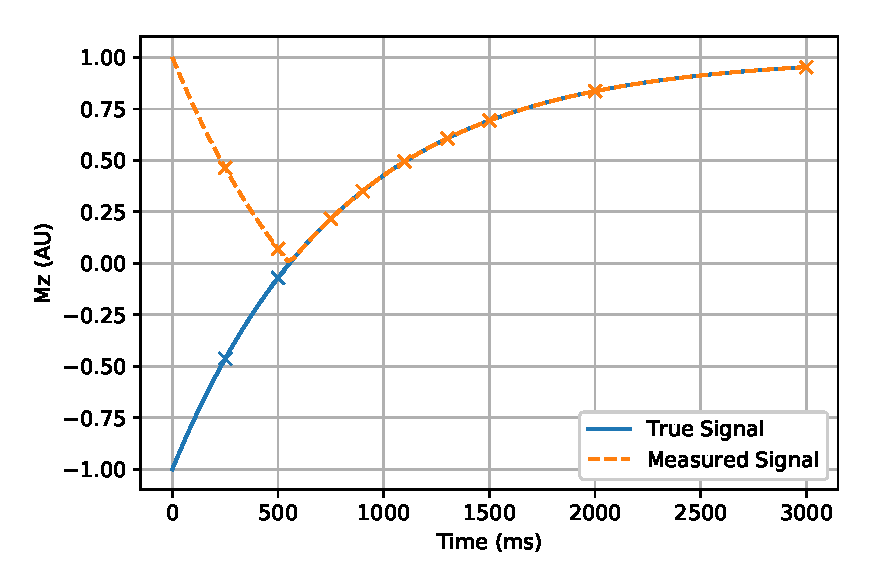
\includegraphics[width=0.5\textwidth]{neph/signal_correction.eps}
	\caption{A simulation of the true and measured magnetisation for a $T_1$ of 800 ms. The crosses represent the inversion times at which the inversion recovery is sampled.}
	\label{fig:sig_correction}	
\end{figure}

Once the data has been polarity corrected a voxel by voxel least squares trust region reflective  method is used to fit the data to Equation \eqref{eq:T1} and estimate the $T_1$ and $M_0$ of the tissue in that voxel along with an uncertainty in the fit \cite{branch_subspace_1999}. This data processing is carried out using an in-house Python package. Once the $T_1$ maps are generated, \ac{ROI} are defined for the renal medulla and renal cortex and the mean $T_1$ in these \ac{ROI} recorded.

\begin{equation}
M_z = M_0 \left(1-2\cdot e^{-TI/T_1}\right)
\label{eq:T1}
\end{equation}

\subsection{$T_2$ Mapping}
\label{subsec:neph_t2_mapping}
There are multiple methods for acquiring $T_2$ maps in the kidneys, \ac{SE}, \ac{ME-TSE}, \ac{GraSE} and $T_2$ preparation. We wish to compare each of these methods in-vivo and verify their accuracy using a calibrated phantom. A QalibreMD System Standard Model 130 \cite{noauthor_system_nodate} is used for verification. All $T_2$ mapping is performed at 3T. 
\subsubsection{Acquisition}

\paragraph{Spin Echo Echo Planar Imaging}

A series of volumes are collected at a range of echo times using a multi-slice spin echo acquisition with \ac{EPI} readout. Acquisition parameters are \ac{FOV} = 288 $\times$ 288 $\times$ 25 mm, voxel size = 3 $\times$ 3 $\times$ 5 mm$^3$, \ac{TR} = 5000 ms, \ac{FA} = $90\degree$, \ac{SENSE} = 2.55, halfscan = 0.844 and the sequence is respiratory triggered for in-vivo use and has an acquisition time of approximately 9 minutes depending on breathing rate. Volumes are acquired at \ac{TE} between 20 ms and 70 ms in 5 ms steps with four volumes being acquired at each echo time. 

\paragraph{Multi-Echo Turbo Spin Echo}

This method also uses a multi-slice spin echo acquisition however unlike the simple spin echo method, uses a multishot \ac{TSE} readout. Acquisition parameters for in-vivo scanning are \ac{FOV} = 288 $\times$ 288 $\times$ 25 mm, voxel size = 3 $\times$ 3 $\times$ 5 mm$^3$, \ac{TR} = 3000 ms, \ac{FA} = $90\degree$, \ac{SENSE} = 2.55 and \ac{TSE} factor = 10; the sequence is respiratory triggered and has an acquisition time of approximately 4 minutes depending on breathing rate. For phantom scanning, the following parameters are modified \ac{FOV} = 250 $\times$ 250 $\times$ 6 mm, voxel size = 0.9 $\times$ 0.9 $\times$ 6 mm$^3$ and respiratory triggering is removed. Volumes are collected with \ac{TE} between 13 ms and 130 ms in 13 ms steps.

\paragraph{Gradient Spin Echo}

This method also uses a multi-slice spin echo acquisition but with a \ac{GraSE} readout. Acquisition parameters for in-vivo scanning are \ac{FOV} = 288 $\times$ 288 $\times$ 25 mm, voxel size = 3 $\times$ 3 $\times$ 5 mm$^3$, \ac{TR} = 3000 ms, \ac{FA} = $90\degree$, \ac{SENSE} = 2.55 and \ac{TSE} factor = 30, startup echoes = 1; the sequence is respiratory triggered and has an acquisition time of approximately 5 minutes depending on breathing rate. For phantom scanning, the following parameters are modified \ac{FOV} = 250 $\times$ 250 $\times$ 6 mm, voxel size = 0.9 $\times$ 0.9 $\times$ 6 mm$^3$ and respiratory triggering is removed. Volumes are collected with \ac{TE} between 11.2 ms and 173.3 ms in 5.6 ms steps.

\paragraph{$T_2$ Preparation}

This technique uses a multi-slice \ac{FFE} acquisition with a \ac{TFEPI} readout. Varying degrees of $T_2$ weighting are applied as a series of $180\degree$ preparation pulses for a variable \ac{eTE}, this is similar to the sequence used in Section \ref{sec:TRUST_MRI}. Acquisition parameters for in-vivo scanning are \ac{FOV} = 288 $\times$ 288 $\times$ 25 mm, voxel size = 3 $\times$ 5.65 $\times$ 5 mm$^3$ (voxel size is limited by the \ac{EPI} factor), \ac{TR} = 3000 ms, \ac{TE} = 5.3, \ac{FA} = $90\degree$, \ac{EPI} factor = 17, \ac{SENSE} = 3 and halfscan = 0.733; the sequence is respiratory triggered and has an acquisition time of approximately 6 minutes depending on breathing rate. As the voxel size is already at its minimum, the only modifications made for scanning the phantom are to decrease the \ac{FOV} to 250 $\times$ 250 $\times$ 6 mm and remove respiratory triggering. \ac{eTE}s of 0, 40, 80 and 160 ms are used with three volumes acquired at each \ac{eTE}

\subsubsection{Analysis}

The data is fit on a voxel by voxel basis using a least squares trust region reflective method to fit the data to Equation \eqref{eq:T2} to estimate $T_2$ and $S_0$ with an uncertainty in the fit \cite{branch_subspace_1999}. For methods where multiple volumes are acquired at an \ac{TE}, individual volumes are used for the fit e.g. four points at each \ac{TE} for the \ac{SE}-\ac{EPI} method rather than taking the mean of the volumes for each \ac{TE}, this makes potential data discarding easier. This post-processing is performed by an in-house Python package. Once the $T_2$ maps have been generated, \ac{ROI} can be defined for different tissue types or phantom compositions.

\begin{equation}
S(t) = S_0 \cdot e^{-t/T_2}
\label{eq:T2}
\end{equation}

\subsection{$T_2^*$ Mapping}
\subsubsection{Acquisition}

Ex-vivo $T_2^*$ maps can be acquired at both 3T and 7T using a multi-slice \ac{FFE} sequence with scans being performed at a range of different echo times. An example of the acquisition at each echo time is shown in Figure \ref{fig:echo_raw_data}

\begin{figure}[H]
	\centering
	%\missingfigure{Individual TE scans}
	\includegraphics[width=0.8\textwidth]{Neph/Individual_TE.eps}
	\caption{Acquisitions at each of the \ac{TE} at 7T.}
	\label{fig:echo_raw_data}	
\end{figure}

The acquisition parameters at 3T are \ac{FOV} = 145 $\times$ 145 $\times$ 15 mm, voxel size = 0.6 $\times$ 0.6 $\times$ 1.5 mm$^3$, \ac{TR} = 697 ms, \ac{FA} = $38\degree$, \ac{SENSE} Factor = 2.0, Acquisition Time $\approx$ 180 sec per \ac{TE} collected. 
The acquisition parameters at 7T are \ac{FOV} = 145 $\times$ 145 $\times$ 10 mm, voxel size = 0.5 $\times$ 0.5 $\times$ 1.0 mm$^3$, \ac{FA} = $38\degree$, \ac{SENSE} Factor = 2.0, Acquisition Time $\approx$ 180 sec per \ac{TE} collected. Initially echo times were 15 ms, 20 ms, 25 ms, 30 ms, 35 ms, 40 ms and 50 ms at 3T and 10 ms, 16 ms, 22 ms, 25 ms, 28 ms and 30 ms at 7T however to reduce acquisition times, the 3T echo times were reduced to 15 ms, 20 ms, 25 ms, 40 ms and 50 ms.

\subsubsection{Analysis}
The data is fit voxel by voxel using a weighted echo time fit from the log of the exponential signal decay (Equation \eqref{eq:T2star}) to generate the $T_2^*$ maps \cite{cox_multiparametric_2017}. This data processing is carried out using an in-house Python package. The \ac{ROI} were defined using the $T_1$ weighted data if available as it has a greater cortical medullary contrast at shorter times from fixation. The mean $T_2^*$ in these \ac{ROI} is recorded.
\begin{equation}
S(t) = S_0 \cdot e^{-TE/T_2^*}
\label{eq:T2star}
\end{equation}

\newpage
\section{Results and Discussion}
\label{sec:neph_results}

\subsection{Fixation and Protocol Development}
As was alluded to in Section \ref{sec:fixation}, there was significant variability in the quality of the samples collected from the slaughterhouse. This was largely due to the legislation surrounding animals slaughtered to enter the human food chain. If any part of the animal is destined for human consumption then the carcase must be thoroughly inspected before any tissue can be released. This can cause two issues. As part of the inspection, the kidneys need to be examined for parasites, this is done by making an incision in the organ, however, the quality of this incision can vary massively with some samples having a 20 mm slice cut into them while others are roughly cut in half. The second issue is caused by the variable time between slaughter and the tissue being released after inspection. For these reasons kidneys began to be procured from Veterinary Science collaborating with Prof David Gardner. The animals slaughtered there are not destined for human consumption and as such the kidneys can be placed into \ac{PBS} and subsequently \ac{NBF} far quicker and the kidneys do not need to be sliced open for inspection. The difference in the samples from these two sources can clearly be seen in Figure \ref{fig:kidney_samples}. This collaboration also enables the procurement of kidneys from a greater range of animals including different ages of pigs and therefore different degrees of fibrosis and inducing \ac{AKI} in the animals prior to scanning and histology. Veterinary Science can also carry out the histology in house, thus streamlining the protocol by avoiding transporting one kidney to Derby for histology and the other to \ac{SPMIC} for scanning.

\begin{figure}[H]
	\centering
	\begin{subfigure}[c]{0.9\textwidth}
		\centering
		\begin{subfigure}[c]{0.47\textwidth}
			\centering
			\includegraphics[width=0.9\textwidth, angle=180]{neph/meat_kidney}
			\caption{}
			\label{fig:meat_kidney}
		\end{subfigure}
		\hfill
		\begin{subfigure}[c]{0.47\textwidth}
			\centering
			\includegraphics[width=0.9\textwidth, angle=180]{neph/sb_kidney}
			\caption{}
			\label{fig:sb_kidney}
		\end{subfigure}
	\end{subfigure}
	\vskip\baselineskip
	\begin{subfigure}[c]{0.9\textwidth}
		\centering
		\begin{subfigure}[c]{0.47\textwidth}
			\centering
			\includegraphics[width=0.9\textwidth]{neph/meat_mri}
			\caption{}
			\label{fig:meat_mri}			
		\end{subfigure}
		\hfill
		\begin{subfigure}[c]{0.47\textwidth}
			\centering
			\includegraphics[width=0.9\textwidth, angle=270]{neph/sb_mri}
			\caption{}
			\label{fig:sb_mri}
		\end{subfigure}
	\end{subfigure}
	\caption{(\subref{fig:meat_kidney}) An example of a sample procured from the slaughterhouse after it has been fixed. The left hand kidney has been sliced in half; the right hand kidney has the incisions from the meat inspector clearly visible. (\subref{fig:sb_kidney}) An example of a sample procured from Veterinary Science post fixing. (\subref{fig:meat_mri}) An example of a $T_2$ weighted FFE with TE = 40 ms of a kidney procured from the slaughterhouse. (\subref{fig:sb_mri}) An example of a $T_2$ weighted FFE with TE = 40 ms of a kidney procured from Veterinary Science.} 
	\label{fig:kidney_samples}
\end{figure}

Once samples had been fixed and transferred to \ac{PBS} they could be placed into the scanner. Using the protocols outlined above it was possible to generate maps as shown in Figure \ref{fig:neph_maps}.

\begin{figure}[H]
	\centering
	\begin{subfigure}[c]{0.9\textwidth}
		\centering
		\begin{subfigure}[c]{0.47\textwidth}
			\centering
			\includegraphics[width=1\textwidth]{Neph/T1_map_3T.eps}
			\caption{}
			\label{fig:neph_t1_map_3t}
		\end{subfigure}
		\hfill
		\begin{subfigure}[c]{0.47\textwidth}
			\centering
			\includegraphics[width=1\textwidth]{Neph/T2star_map_3T.eps}
			\caption{}
			\label{fig:neph_t2star_map_3t}
		\end{subfigure}
	\end{subfigure}
	\vskip\baselineskip
	\begin{subfigure}[c]{0.9\textwidth}
		\centering
		\begin{subfigure}[c]{0.47\textwidth}
			\centering
			\includegraphics[width=1\textwidth]{Neph/T1_map_7T.eps}
			\caption{}
			\label{fig:neph_t1_map_7t}			
		\end{subfigure}
		\hfill
		\begin{subfigure}[c]{0.47\textwidth}
			\centering
			\includegraphics[width=1\textwidth]{Neph/T2star_map_7T.eps}
			\caption{}
			\label{fig:neph_t2star_map_7t}
		\end{subfigure}
	\end{subfigure}
	\caption{(\subref{fig:neph_t1_map_3t}) $T_1$ map of a kidney twenty four hours after fixation at 3T (\subref{fig:neph_t2star_map_3t}) $T_2^*$ map twenty four hours after fixation at 3T (\subref{fig:neph_t1_map_7t}) $T_1$ map twenty four hours after fixation at 7T (\subref{fig:neph_t2star_map_7t}) $T_2^*$ map twenty four hours after fixation at 7T. The sample shown in the 3T and 7T figures is different.} 
	\label{fig:neph_maps}
\end{figure}

\subsection{Monitoring Changes in MR Parameters Post Fixation}
\label{sec:longevity}
To study the effects of the fixation process upon MR measurements, a kidney was fixed as per the method in Section \ref{sec:fixation} and scanned at both field strengths of 3T and 7T. Collecting a $T_1$ and $T_2^*$ map took approximately 90 minutes per field strength. Once the maps had been generated, \ac{ROI} were defined and the mean $T_1$ and $T_2^*$ for the cortex and the medulla were calculated. The sample was monitored for ten weeks. The variation in $T_1$ and $T_2^*$ over time can be seen in Figure \ref{fig:fixation_lts}.\\

\begin{figure}[H]
	\centering
	\begin{subfigure}[c]{0.9\textwidth}
		\centering
		\begin{subfigure}[c]{0.47\textwidth}
			\centering
			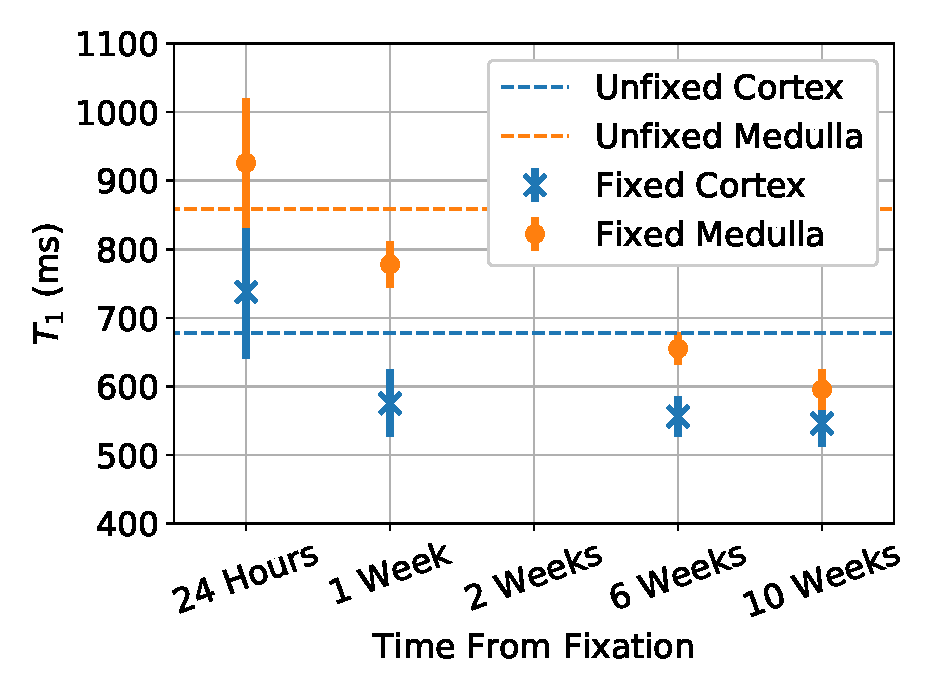
\includegraphics[width=1\textwidth]{Neph/T1_3T_crop.eps}
			\caption{}
			\label{fig:fixation_t1_3t_lts}
		\end{subfigure}
		\hfill
		\begin{subfigure}[c]{0.47\textwidth}
			\centering
			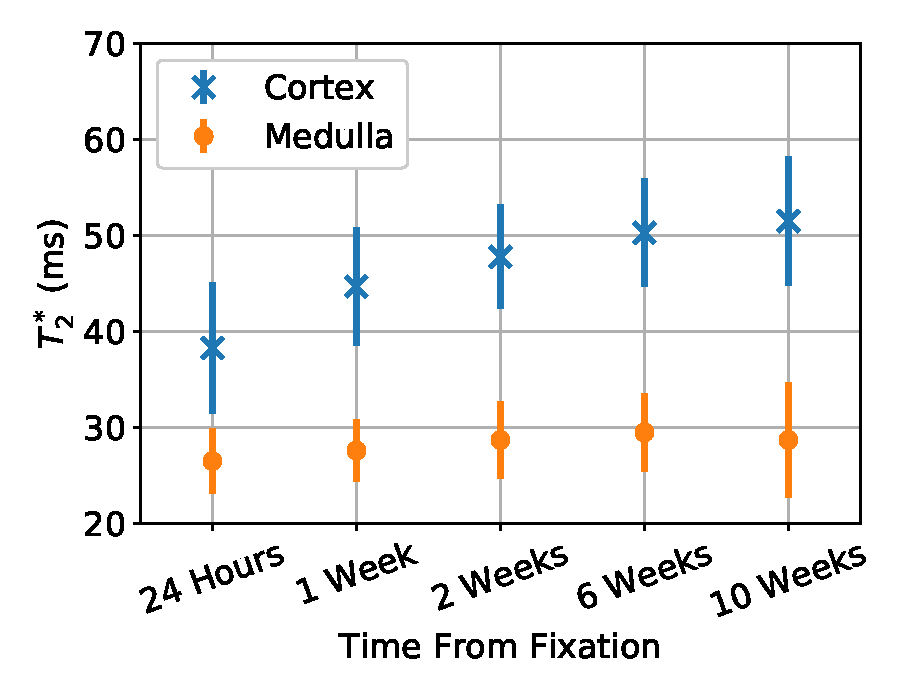
\includegraphics[width=1\textwidth]{Neph/T2star_3T_crop.eps}
			\caption{}
			\label{fig:fixation_t2star_3t_lts}
		\end{subfigure}
	\end{subfigure}
	\vskip\baselineskip
	\begin{subfigure}[c]{0.9\textwidth}
		\centering
		\begin{subfigure}[c]{0.47\textwidth}
			\centering
			\includegraphics[width=1\textwidth]{Neph/T1_7T_crop.eps}
			\caption{}
			\label{fig:fixation_t1_7t_lts}
		\end{subfigure}
		\hfill
		\begin{subfigure}[c]{0.47\textwidth}
			\centering
			\includegraphics[width=1\textwidth]{Neph/T2star_7T_crop.eps}
			\caption{}
			\label{fig:fixation_t2star_7t_lts}
		\end{subfigure}
	\end{subfigure}
	\caption{(\subref{fig:fixation_t1_3t_lts}) Variation in $T_1$ as a function of time after fixation measured at 3T (\subref{fig:fixation_t2star_3t_lts}) Variation in $T_2^*$ as a function of time after fixation measured at 3T (\subref{fig:fixation_t1_7t_lts}) Variation in $T_1$ as a function of time after fixation measured at 7T (\subref{fig:fixation_t2star_7t_lts})  Variation in $T_2^*$ as a function of time after fixation measured at 7T.}
	\label{fig:fixation_lts}
\end{figure}

Unfortunately due to technical scanner issues, we were not able to scan the sample at 7T at ten weeks and the quality of the 3T $T_1$ acquisition at two weeks was significantly inferior; as such these data points have been omitted. It can be seen that the largest changes in $T_1$ and $T_2^*$ occur between twenty four hours and one week after fixation, after that there is a general trend that the $T_1$ of the cortex and medulla converge while the $T_2^*$ of each tissue type diverges, one could argue that the $T_2^*$ of the cortex measured at 3T is plateauing. This means that, although the samples will reach a steady state, in the first few weeks after fixation, their $T_1$ and $T_2^*$ will have a dependence on time. This necessitates the need to standardise the protocol, specifically the time at which the samples are scanned. It would have been useful to know the $T_1$ and $T_2^*$ of unfixed porcine kidneys and as such, a fresh, unfixed kidney was scanned using the same protocol. Unfortunately, due to the difference in stiffness between fixed and unfixed kidneys, the same protocol did not deliver usable $T_2^*$ data as the unfixed kidney vibrated too much while floating in the \ac{PBS}. This problem could potentially be reduced by either vibration insulation between the sample and the scanner as per Dawe et al \cite{dawe_postmortem_nodate} or by embedding the sample in an agarose medium rather than allowing it to float in \ac{PBS} as per Kolk et al\cite{kolk_imaging_2014}. The $T_1$ of the unfixed kidney was seen to be between that of the fixed kidney between 24-hours and one week.\\

To investigate this time dependence over a shorter time scale, a pair of kidneys were acquired and fixed as before. It will be possible to scan most human samples within 24 hours of fixation, as such it is desirable to see how much $T_1$, $T_2^*$ and histology change over this period. Scanning was only carried out at 3T as more frequent measurements were preferable to measurements at different field strengths. For this reason the number of inversion times and echo times used to generate the $T_1$ and $T_2^*$ maps was reduced to \ac{TI} = 400 ms, 500 ms, 750 ms, 900 ms, 1100 ms, 2600 ms and \ac{TE} = 15 ms, 20 ms, 25 ms, 40 ms, 50 ms respectively. The choice of these inversion/echo times was arrived at empirically by carrying out the analysis pipeline on a single slice of data using each combination of six and five of the previously used \ac{TI}s and \ac{TE}s respectively. The results from each combination of \ac{TI}/\ac{TE} were compared to those generated when using the full complement of inversion/echo times and the combination delivering the minimum difference chosen. This reduction in the number of inversion times resulted in a mean error per voxel in the kidney of 20.9 $\pm$ 12.3 ms if the full complement of inversion times was taken as the ground truth, the reduction in echo times resulted in a mean error of 0.3 $\pm$ 1.2 ms.\\

Scanning sessions started at 1.5 hours, 2.5 hours, 4 hours, 5.5 hours, 19 hours and 22 hours after the sample was removed from the \ac{NBF}. Due to the potential for the properties to change relatively quickly, especially $T_1$, it was decided to randomise the order in which the inversion/echo times were collected, this way any change in $T_1$/$T_2^*$ over the 30/20 minute acquisition period would manifest itself as non-systematic noise and thus will increase the uncertainty in the fit rather than affecting the predicted value. At the start of each scanning session, a biopsy was performed on the kidney not being scanned. Masson's trichrome and \ac{H and E} staining was performed on these samples.\\

\begin{figure}[H]
	\centering
	\begin{subfigure}[c]{0.47\textwidth}
		\centering
%		\missingfigure{T1 vs Times (STS)}
		\includegraphics[width=1\textwidth]{Neph/STS_T1_line.eps}
		\caption{}
		\label{fig:fixation_t1_3t_sts}
	\end{subfigure}
	\hfill
	\begin{subfigure}[c]{0.47\textwidth}
		\centering
%		\missingfigure{T2* vs Times (STS)}
		\includegraphics[width=1\textwidth]{Neph/STS_T2star_line.eps}
		\caption{}
		\label{fig:fixation_t2star_3t_sts}
	\end{subfigure}
	\caption{(\subref{fig:fixation_t1_3t_sts}) Variation in $T_1$ as a function of time after fixation measured at 3T (\subref{fig:fixation_t2star_3t_sts}) Variation in $T_2^*$ as a function of time after fixation measured at 3T.}
	\label{fig:fixation_sts}
\end{figure}

No significant change in $T_1$ or $T_2^*$ was observed over the period the sample was monitored. This is promising as it means that when this protocol is applied to human samples, there will be a relatively large time window in which the ex-vivo scan can be carried out, making the experimental procedure simpler. The corresponding histology results showed no change in the cortex over this period however there was a noticeable inflammatory response in the medulla.\\

It was noted that the sample used for this experiment was not of especially high quality, the kidney has two slices in it, one that almost bifurcated the sample along the coronal plane, another cut down one half of the sample along the sagittal plane, visible in Figure \ref{fig:fixation_t1map_3t_sts}. These cuts meant that air became trapped within the sample causing it to float in the \ac{PBS}. If not corrected this would cause large susceptibility artefacts where the sample came into contact with the air at the top of the \ac{PBS}; to remedy this the sample was entirely bifurcated. Despite the best efforts of investigators, air bubbles remained in the sagittal slice, causing the aforementioned artefacts, especially visible in Figure \ref{fig:fixation_t2starmap_3t_sts}. Given these concerns over sample quality, it was decided to scan the sample again one week after fixation, to match the time period in the previous experiment (Figure \ref{fig:fixation_lts}).\\

\begin{figure}[H]
	\centering
	\begin{subfigure}[c]{0.47\textwidth}
		\centering
		\includegraphics[width=1\textwidth]{Neph/T1_map_STS.eps}
		\caption{}
		\label{fig:fixation_t1map_3t_sts}
	\end{subfigure}
	\hfill
	\begin{subfigure}[c]{0.47\textwidth}
		\centering
		\includegraphics[width=1\textwidth]{Neph/T2star_map_STS.eps}
		\caption{}
		\label{fig:fixation_t2starmap_3t_sts}
	\end{subfigure}
	\caption{(\subref{fig:fixation_t1map_3t_sts}) An example of the $T_1$ map collected from the short time scale kidney (\subref{fig:fixation_t2starmap_3t_sts}) An example of the $T_2^*$ map collected from the short time scale kidney.}
	\label{fig:neph_maps_sts}
\end{figure}

It was expected that upon repeating the measurements one week later, the $T_1$ of both cortex and medulla would decrease and the $T_2^*$ of the cortex would increase. This was not the case, there was a slight decrease in the $T_1$ of the medulla but otherwise, no change was observed, Figure \ref{fig:fixation_mts}. This lead us to conclude that the large cuts in the sample had lead to a different level of fixation. Subsequent to this, samples were to be procured from Veterinary Science as they are more consistent and therefore more akin to the human samples that will be used.\\

\begin{figure}[H]
	\centering
	\begin{subfigure}[c]{0.47\textwidth}
		\centering
%		\missingfigure{T1 vs Times (MTS)}
		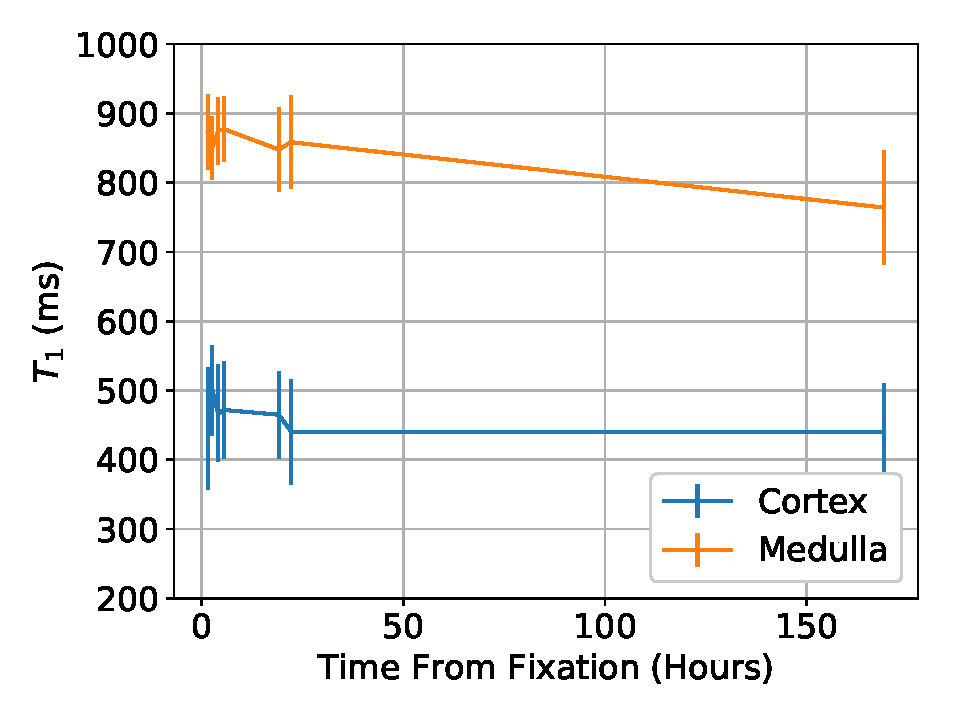
\includegraphics[width=1\textwidth]{Neph/MTS_T1_line.eps}
		\caption{}
		\label{fig:fixation_t1_3t_mts}
	\end{subfigure}
	\hfill
	\begin{subfigure}[c]{0.47\textwidth}
		\centering
%		\missingfigure{T2* vs Times (MTS)}
		\includegraphics[width=1\textwidth]{Neph/MTS_T2star_line.eps}
		\caption{}
		\label{fig:fixation_t2star_3t_mts}
	\end{subfigure}
	\caption{(\subref{fig:fixation_t1_3t_mts}) Variation in $T_1$ as a function of time after fixation measured at 3T (\subref{fig:fixation_t2star_3t_mts}) Variation in $T_2^*$ as a function of time after fixation measured at 3T.}
	\label{fig:fixation_mts}
\end{figure}

\subsection{Comparing MR and Histological Measures in Aged Kidneys}

To verify the correlation of MR measurements with histology, kidneys were collected from a 0.5 year old and 2.5 year old pig. These different ages were expected to have differing levels of renal inflammation and fibrosis. Figure \ref{fig:aged_map} shows example \ac{MRI} data collected from these samples, Figure \ref{fig:aged_bar} shows the quantitative differences in $T_1$ and $T_2^*$ between the two samples.

\begin{figure}[H]
	\centering
	\begin{subfigure}[c]{0.47\textwidth}
		\centering
		\includegraphics[width=1\textwidth]{Neph/aged_kidneys/Young_T1.eps}
		\caption{}
		\label{fig:neph_aged_t1_map}
	\end{subfigure}
	\hfill
	\begin{subfigure}[c]{0.47\textwidth}
		\centering
		\includegraphics[width=1\textwidth]{Neph/aged_kidneys/Old_T1.eps}
		\caption{}
		\label{fig:neph_aged_t2star_map}
	\end{subfigure}
	\caption{(\subref{fig:neph_aged_t1_map}) $T_1$ map of a 0.5 year old pig kidney. (\subref{fig:neph_aged_t2star_map}) $T_1$ map of a 2.5 year old pg kidney.}
	\label{fig:aged_map}
\end{figure}

\begin{figure}[H]
	\centering
	\begin{subfigure}[c]{0.47\textwidth}
		\centering
		\includegraphics[width=1\textwidth]{Neph/aged_kidneys/T1_bar.eps}
		\caption{}
		\label{fig:neph_aged_t1_bar}
	\end{subfigure}
	\hfill
	\begin{subfigure}[c]{0.47\textwidth}
		\centering
		\includegraphics[width=1\textwidth]{Neph/aged_kidneys/T2star_bar.eps}
		\caption{}
		\label{fig:neph_aged_t2star_bar}
	\end{subfigure}
	\caption{(\subref{fig:neph_aged_t1_bar}) The $T_1$ of the renal cortex and medulla of the two samples. (\subref{fig:neph_aged_t2star_bar}) The $T_2^*$ of the renal cortex and medulla of the two samples.}
	\label{fig:aged_bar}
\end{figure}

No significant change is observed in the $T_1$ or $T_2^*$ of cortex the two kidneys. There is however a decrease in $T_1$ seen in the medulla of the older kidney. Cortical samples were removed from the same animals for histological analysis. These samples were stained using \ac{H and E} and Masson's trichrome to enable the evaluation of levels of fibrosis, these micrographs are shown in Figure \ref{fig:aged_histo}. 

\begin{figure}[H]
	\centering
	\begin{subfigure}[c]{0.9\textwidth}
		\centering
		\begin{subfigure}[c]{0.47\textwidth}
			\centering
			\includegraphics[width=1\textwidth]{Neph/aged_kidneys/Figure_5_V3_Young_H_and_E.png}
			\caption{}
			\label{fig:neph_young_h_and_e}
		\end{subfigure}
		\hfill
		\begin{subfigure}[c]{0.47\textwidth}
			\centering
			\includegraphics[width=1\textwidth]{Neph/aged_kidneys/Figure_5_V3_Old_H_and_E.png}
			\caption{}
			\label{fig:neph_old_h_and_e}
		\end{subfigure}
	\end{subfigure}
	\vskip\baselineskip
	\begin{subfigure}[c]{0.9\textwidth}
		\centering
		\begin{subfigure}[c]{0.47\textwidth}
			\centering
			\includegraphics[width=1\textwidth]{Neph/aged_kidneys/Figure_5_V3_Young_Trichrome.png}
			\caption{}
			\label{fig:neph_young_trichrome}			
		\end{subfigure}
		\hfill
		\begin{subfigure}[c]{0.47\textwidth}
			\centering
			\includegraphics[width=1\textwidth]{Neph/aged_kidneys/Figure_5_V3_Old_Trichrome.png}
			\caption{}
			\label{fig:neph_old_trichrome}
		\end{subfigure}
	\end{subfigure}
	\caption{(\subref{fig:neph_young_h_and_e}) A sample of renal cortex from a 0.5 year old pig stained with \ac{H and E}. (\subref{fig:neph_old_h_and_e}) A sample of renal cortex from a 2.5 year old pig stained with \ac{H and E}. (\subref{fig:neph_young_trichrome}) A sample of renal cortex from a 0.5 year old pig stained with Masson's trichrome. (\subref{fig:neph_old_trichrome}) A sample of renal cortex from a 2.5 year old pig stained with Masson's trichrome.} 
	\label{fig:aged_histo}
\end{figure}

No significant difference is seen between the histology of these cortical samples. This means that \ac{MRI} and histology are in agreement. Unfortunately no samples were taken from the renal medulla, the area which showed a change in MR measurements. In future samples with a larger difference in age should be used as these will have a greater difference in fibrosis and samples should be taken from the medulla for histological analysis.

\subsection{Comparison of $T_2$ Mapping Methods}

\subsubsection{Quantitative Phantom}

We began by comparing the quantitative accuracy of each of the proposed $T_2$ mapping methods (spin echo \ac{EPI}, multi-echo \ac{TSE}, \ac{GraSE} and $T_2$ preparation).  The QalibreMD System Standard Model 130 phantom used has fourteen spheres with $T_2$ between 5.35 ms and 645.8 ms spanning the range of $T_2$ expected in the kidneys, Figure \ref{fig:neph_phantom_eg}. This phantom was scanned using each of the methods outlined in \ref{subsec:neph_t2_mapping} and a \ac{ROI} defined for each sphere. 

\begin{figure}[H]
	\centering
	\begin{subfigure}[c]{0.47\textwidth}
		\centering
		\includegraphics[width=1\textwidth]{Neph/T2_methods/Phantom_Example/Localiser_multi.eps}
		\caption{}
		\label{fig:neph_phantom_loc}
	\end{subfigure}
	\hfill
	\begin{subfigure}[c]{0.47\textwidth}
		\centering
		\includegraphics[width=1\textwidth]{Neph/T2_methods/Phantom_Example/GraSE_map_0_500.eps}
		\caption{}
		\label{fig:neph_phantom_map}
	\end{subfigure}
	\caption{(\subref{fig:neph_phantom_loc}) The $T_2$ spheres inside the phantom. (\subref{fig:neph_phantom_map}) An example $T_2$ map, in this case generated using the \ac{GraSE} method.}
	\label{fig:neph_phantom_eg}
\end{figure}

The spin echo method produced vastly over-estimated readings for the spheres of $T_2$ less than 20 ms (Figures \ref{fig:neph_phantom_se_mean}) due to the longer minimum \ac{TE} compared to the other methods. This can be seen in Figure \ref{fig:neph_phantom_se_raw} where the signal from the shortest $T_2$ spheres has already mostly decayed. This method did however deliver accurate measurements for the remaining spheres.\\

More accurate results were generated for shorter $T_2$ spheres using the \ac{ME-TSE} method. The raw data (Figure \ref{fig:neph_phantom_metse_raw}) is more noisy, with a sawtooth pattern visible, this additional noise manifests itself as inaccuracies in the longer $T_2$ measurements where the dynamic range over the \ac{TE} sampled is smaller.\\

The \ac{GraSE} method produced the most accurate measurements although still struggled to measure the sphere with a $T_2$ of 5.35 ms, Figure \ref{fig:neph_phantom_grase_mean}. The large range of \ac{TE} and number of volumes collected means this method produced the most accurate results. It also has the benefit of being able to be performed at high resolutions with voxel sizes of 0.9 x 0.9 mm unlike the \ac{SE}-\ac{EPI} and $T_2$ prep methods; this makes it well suited to both in-vivo and ex-vivo measurements.\\

The data collected using the $T_2$ prep method (Figures \ref{fig:neph_phantom_t2prep_raw} and \ref{fig:neph_phantom_t2prep_mean}) did not fit well due to its small number of data points and large degradation in image quality.\\

\begin{figure}[H]
	\centering
	\begin{subfigure}[c]{0.9\textwidth}
		\centering
		\begin{subfigure}[c]{0.47\textwidth}
			\centering
			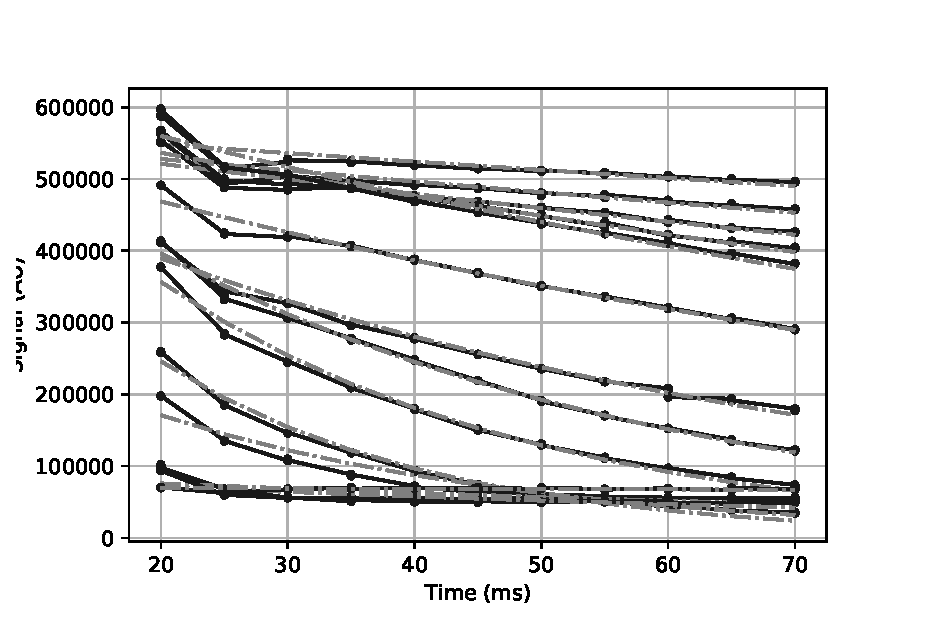
\includegraphics[width=1\textwidth]{Neph/T2_methods/Phantom/SE_raw.eps}
			\caption{}
			\label{fig:neph_phantom_se_raw}
		\end{subfigure}
		\hfill
		\begin{subfigure}[c]{0.47\textwidth}
			\centering
			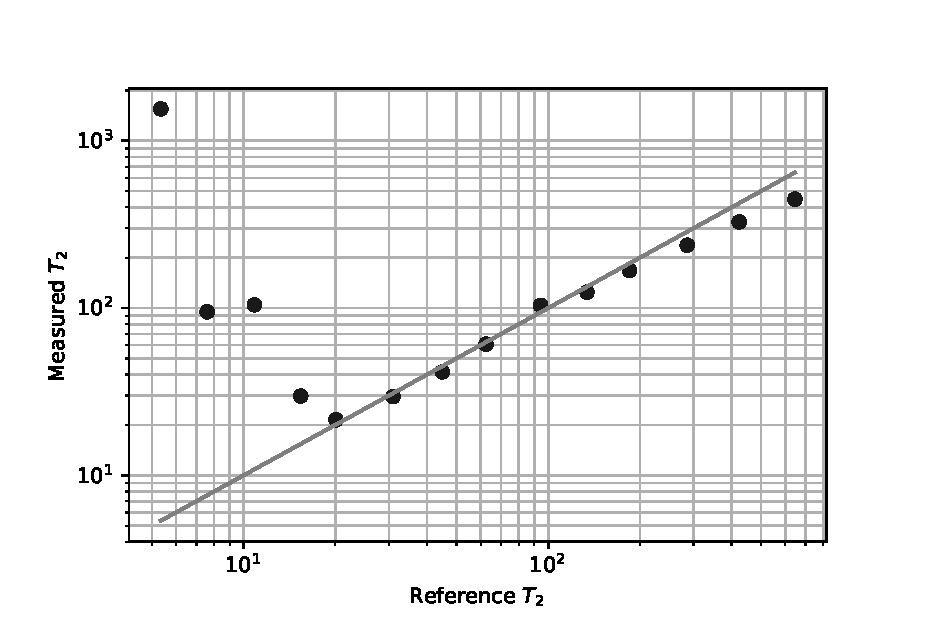
\includegraphics[width=1\textwidth]{Neph/T2_methods/Phantom/SE_mean.eps}
			\caption{}
			\label{fig:neph_phantom_se_mean}
		\end{subfigure}
	\end{subfigure}
	\vskip\baselineskip
	\begin{subfigure}[c]{0.9\textwidth}
		\centering
		\begin{subfigure}[c]{0.47\textwidth}
			\centering
			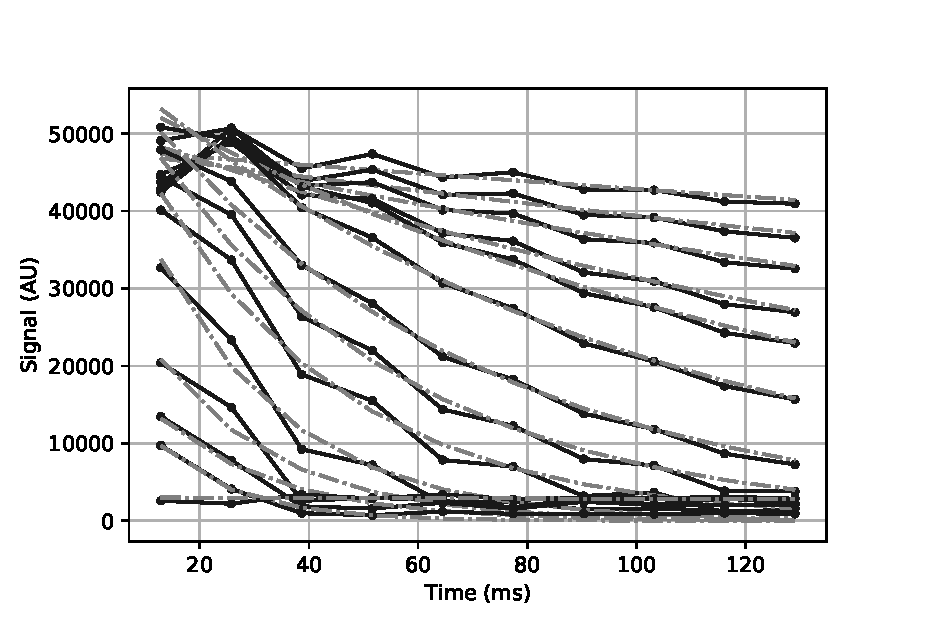
\includegraphics[width=1\textwidth]{Neph/T2_methods/Phantom/METSE_HR_raw.eps}
			\caption{}
			\label{fig:neph_phantom_metse_raw}
		\end{subfigure}
		\hfill
		\begin{subfigure}[c]{0.47\textwidth}
			\centering
			\includegraphics[width=1\textwidth]{Neph/T2_methods/Phantom/METSE_HR_mean.eps}
			\caption{}
			\label{fig:neph_phantom_metse_mean}
		\end{subfigure}
	\end{subfigure}
	\vskip\baselineskip
	\begin{subfigure}[c]{0.9\textwidth}
		\centering
		\begin{subfigure}[c]{0.47\textwidth}
			\centering
			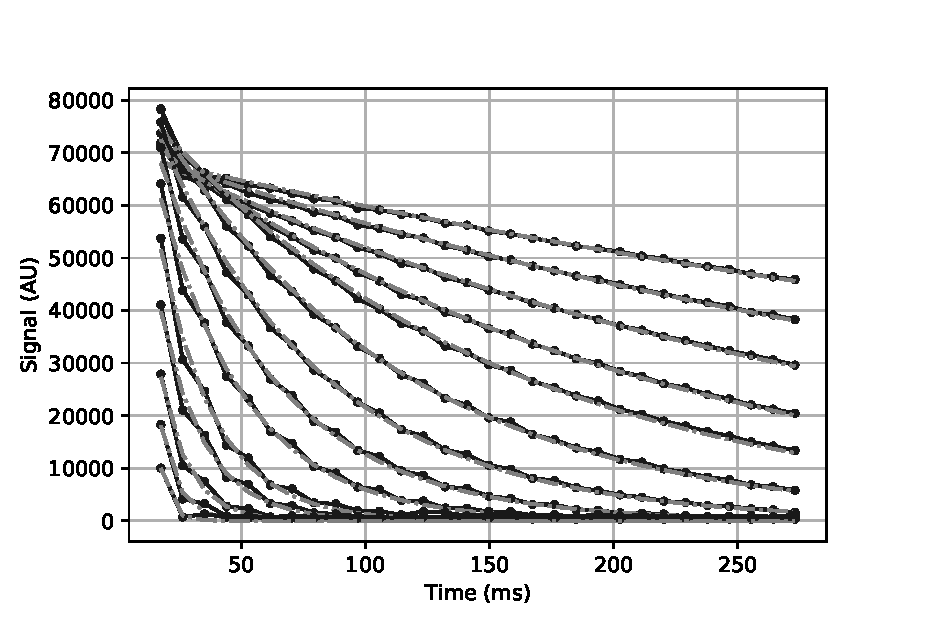
\includegraphics[width=1\textwidth]{Neph/T2_methods/Phantom/GraSE_HR_raw.eps}
			\caption{}
			\label{fig:neph_phantom_grase_raw}
		\end{subfigure}
		\hfill
		\begin{subfigure}[c]{0.47\textwidth}
			\centering
			\includegraphics[width=1\textwidth]{Neph/T2_methods/Phantom/GraSE_HR_mean.eps}
			\caption{}
			\label{fig:neph_phantom_grase_mean}
		\end{subfigure}
	\end{subfigure}
	\vskip\baselineskip
	\begin{subfigure}[c]{0.9\textwidth}
		\centering
		\begin{subfigure}[c]{0.47\textwidth}
			\centering
			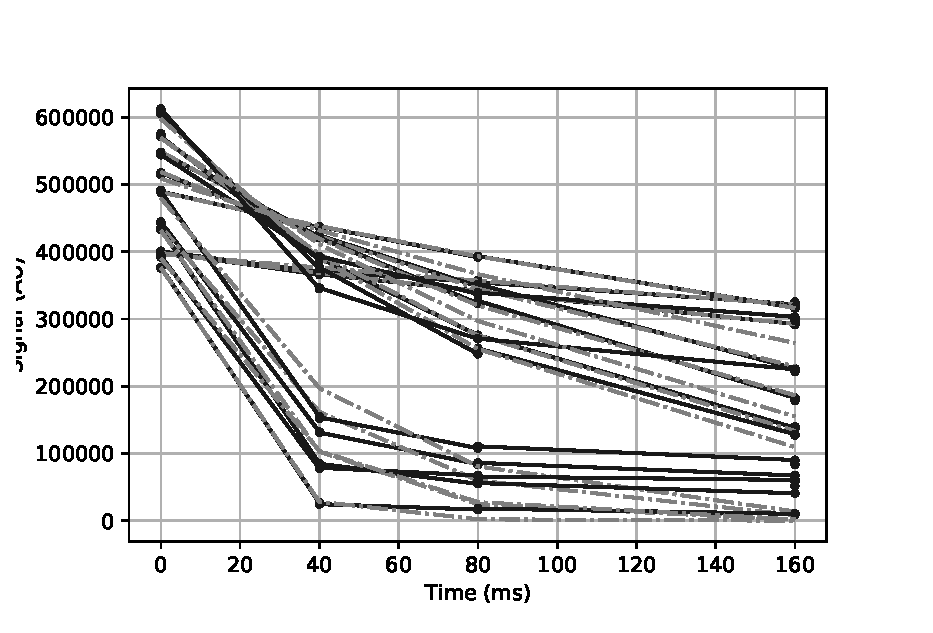
\includegraphics[width=1\textwidth]{Neph/T2_methods/Phantom/T2prep_raw.eps}
			\caption{}
			\label{fig:neph_phantom_t2prep_raw}
		\end{subfigure}
		\hfill
		\begin{subfigure}[c]{0.47\textwidth}
			\centering
			\includegraphics[width=1\textwidth]{Neph/T2_methods/Phantom/T2prep_mean.eps}
			\caption{}
			\label{fig:neph_phantom_t2prep_mean}
		\end{subfigure}
	\end{subfigure}
	\caption{Figures (\subref{fig:neph_phantom_se_raw}), (\subref{fig:neph_phantom_metse_raw}), (\subref{fig:neph_phantom_grase_raw}) and (\subref{fig:neph_phantom_t2prep_raw}) show the raw signal decay for each of the fourteen spheres and the fit decay. Figures (\subref{fig:neph_phantom_se_mean}), (\subref{fig:neph_phantom_metse_mean}), (\subref{fig:neph_phantom_grase_mean}) and (\subref{fig:neph_phantom_t2prep_mean}) show how the fit $T_2$ compares to the literature value. Figures (\subref{fig:neph_phantom_se_raw}) and (\subref{fig:neph_phantom_se_mean}) show the results from the \ac{SE}-\ac{EPI} method, (\subref{fig:neph_phantom_metse_raw}) and (\subref{fig:neph_phantom_metse_mean}) show the results form the \ac{ME-TSE} method, (\subref{fig:neph_phantom_grase_raw}) and (\subref{fig:neph_phantom_grase_mean}) show the results form the \ac{GraSE} method and (\subref{fig:neph_phantom_t2prep_raw}) and (\subref{fig:neph_phantom_t2prep_mean}) show the results from the $T_2$ prep method.} 
	\label{fig:neph_phantom}
\end{figure}


\subsubsection{In-Vivo}

$T_2$ maps using all four methods were collected on the same subject in the same scanning session to allow for a direct comparison of the in-vivo data.\\ 

\begin{figure}[H]
	\centering
	\begin{subfigure}[c]{0.9\textwidth}
		\centering
		\begin{subfigure}[c]{0.47\textwidth}
			\centering
			\includegraphics[width=1\textwidth]{Neph/T2_methods/SE/SE_Raw_Echoes.eps}
			\caption{}
			\label{fig:neph_t2_se_raw}
		\end{subfigure}
		\hfill
		\begin{subfigure}[c]{0.47\textwidth}
			\centering
			\includegraphics[width=1\textwidth]{Neph/T2_methods/SE/SE_Map.eps}
			\caption{}
			\label{fig:neph_t2_se_map}
		\end{subfigure}
	\end{subfigure}
	\vskip\baselineskip
	\begin{subfigure}[c]{0.9\textwidth}
		\centering
		\includegraphics[width=1\textwidth]{Neph/T2_methods/SE/SE_Decay.eps}
		\caption{}
		\label{fig:neph_t2_se_decay}			
	\end{subfigure}
	\caption{(\subref{fig:neph_t2_se_raw}) The raw data used to generate the \ac{SE}-\ac{EPI} $T_2$ map.  (\subref{fig:neph_t2_se_map}) An example slice from the \ac{SE}-\ac{EPI} $T_2$ map. (\subref{fig:neph_t2_se_decay}) The signal decay for the renal cortex and medulla.} 
	\label{fig:neph_t2_se}
\end{figure}

The \ac{SE}-\ac{EPI} method (Figure \ref{fig:neph_t2_se}) generated maps with little blurring however there is also a lack of differentiation in $T_2$ between the renal cortex and medulla. The data collected at \ac{TE} of 20 ms appears to be artificially high and leads to a reduction in fit $T_2$. This sequence is the most susceptible of the methods to patient motion due to the acquisition method of a series per \ac{TE}, this increase in motion is clear when scrolling through \ac{TE}. 

\begin{figure}[H]
	\centering
	\begin{subfigure}[c]{0.9\textwidth}
		\centering
		\begin{subfigure}[c]{0.47\textwidth}
			\centering
			\includegraphics[width=1\textwidth]{Neph/T2_methods/ME/ME_Raw_Echoes.eps}
			\caption{}
			\label{fig:neph_t2_me_raw}
		\end{subfigure}
		\hfill
		\begin{subfigure}[c]{0.47\textwidth}
			\centering
			\includegraphics[width=1\textwidth]{Neph/T2_methods/ME/ME_Map.eps}
			\caption{}
			\label{fig:neph_t2_me_map}
		\end{subfigure}
	\end{subfigure}
	\vskip\baselineskip
	\begin{subfigure}[c]{0.9\textwidth}
		\centering
		\includegraphics[width=1\textwidth]{Neph/T2_methods/ME/ME_Decay.eps}
		\caption{}
		\label{fig:neph_t2_me_decay}			
	\end{subfigure}
	\caption{(\subref{fig:neph_t2_me_raw}) The raw data used to generate the \ac{ME-TSE} $T_2$ map.  (\subref{fig:neph_t2_me_map}) An example slice from the \ac{ME-TSE} $T_2$ map. (\subref{fig:neph_t2_me_decay}) The signal decay for the renal cortex and medulla.} 
	\label{fig:neph_t2_me}
\end{figure}

The map generated by the \ac{ME-TSE} method (Figure \ref{fig:neph_t2_me}) suffers from a large amount of blurring due to the relatively long echo train length. The number of echoes acquired is limited to the \ac{TSE} factor therefore to acquire ten echoes, a \ac{TSE} factor of ten needs to be used. This blurring leads to structures being obscured in the map and only a very small differentiation between cortex and medulla.

\begin{figure}[H]
	\centering
	\begin{subfigure}[c]{0.9\textwidth}
		\centering
		\begin{subfigure}[c]{0.47\textwidth}
			\centering
			\includegraphics[width=1\textwidth]{Neph/T2_methods/GraSE/GraSE_Raw_Echoes.eps}
			\caption{}
			\label{fig:neph_t2_grase_raw}
		\end{subfigure}
		\hfill
		\begin{subfigure}[c]{0.47\textwidth}
			\centering
			\includegraphics[width=1\textwidth]{Neph/T2_methods/GraSE/GraSE_Map.eps}
			\caption{}
			\label{fig:neph_t2_grase_map}
		\end{subfigure}
	\end{subfigure}
	\vskip\baselineskip
	\begin{subfigure}[c]{0.9\textwidth}
		\centering
		\includegraphics[width=1\textwidth]{Neph/T2_methods/GraSE/GraSE_Decay.eps}
		\caption{}
		\label{fig:neph_t2_grase_decay}			
	\end{subfigure}
	\caption{(\subref{fig:neph_t2_grase_raw}) The raw data used to generate the \ac{GraSE} $T_2$ map.  (\subref{fig:neph_t2_grase_map}) An example slice from the \ac{GraSE} $T_2$ map. (\subref{fig:neph_t2_grase_decay}) The signal decay for the renal cortex and medulla.}
	\label{fig:neph_t2_grase}
\end{figure}

Using the \ac{GraSE} method the data in Figure \ref{fig:neph_t2_grase} was collected. There is a clear difference between cortical and medullary $T_2$ and the data fits well to a $T_2$ decay (Figure \ref{fig:neph_t2_grase_decay}). The signal from the first echo in Figure \ref{fig:neph_t2_grase_decay} is too intense, this effect was even more pronounced when no startup echoes were used. For tissues with a longer $T_2$ using two startup echoes would be preferable however this makes measurements of tissues with a short $T_2$ more inaccurate, as such a compromise of a single startup echo was used. The short echo-spacing made possible by \ac{GraSE} means more \ac{TE} can be sampled and therefore leads to a more accurate fit.

\begin{figure}[H]
	\centering
	\begin{subfigure}[c]{0.9\textwidth}
		\centering
		\begin{subfigure}[c]{0.47\textwidth}
			\centering
			\includegraphics[width=1\textwidth]{Neph/T2_methods/T2prep/T2prep_Raw_Echoes.eps}
			\caption{}
			\label{fig:neph_t2_t2prep_raw}
		\end{subfigure}
		\hfill
		\begin{subfigure}[c]{0.47\textwidth}
			\centering
			\includegraphics[width=1\textwidth]{Neph/T2_methods/T2prep/T2prep_Map.eps}
			\caption{}
			\label{fig:neph_t2_t2prep_map}
		\end{subfigure}
	\end{subfigure}
	\vskip\baselineskip
	\begin{subfigure}[c]{0.9\textwidth}
		\centering
		\includegraphics[width=1\textwidth]{Neph/T2_methods/T2prep/T2prep_Decay.eps}
		\caption{}
		\label{fig:neph_t2_t2prep_decay}			
	\end{subfigure}
	\caption{(\subref{fig:neph_t2_t2prep_raw}) The mean data at each \ac{eTE} used to generate the $T_2$ preparation $T_2$ map.  (\subref{fig:neph_t2_t2prep_map}) An example slice from the $T_2$ preparation $T_2$ map. (\subref{fig:neph_t2_t2prep_decay}) The signal decay for the renal cortex and medulla.} 
	\label{fig:neph_t2_t2prep}
\end{figure}

The map made using the $T_2$ preparation method (Figure \ref{fig:neph_t2_t2prep}) suffers from noise in the raw data, this is despite there being three acquisitions at each \ac{eTE}. When comparing Figure \ref{fig:neph_t2_t2prep_map} to Figure \ref{fig:neph_t2_grase_map} it's possible to see that some of the areas of greater $T_2$ do match with the medulla, however the degree of noise in \ref{fig:neph_t2_t2prep_map} means it is un-usable on its own. The small number of \ac{eTE} collected means the uncertainty in the fit $T_2$ is higher for this method.\\

The two methods that have delivered the highest image quality, \ac{SE}-\ac{EPI} and \ac{GraSE}, produce substantially different values of $T_2$ in-vivo. Even when the data from the 20 ms volume is omitted from the \ac{SE}-\ac{EPI} fit, the $T_2$ is far lower. This is surprising give that when deployed on the phantom, this protocol delivered accurate results over the range of $T_2$ we see in the kidneys. This disparity is due to the additional confounding factors of diffusion and flow that are present in the body. These factors do not affect the \ac{GraSE} sequence to the same degree as the \ac{SE}-\ac{EPI} sequence.\\

Of the methods explored, the \ac{GraSE} sequence produced the most accurate results on the phantom and superior image quality in-vivo, we will use this sequence in $T_2$ mapping going forward.

\section{Conclusions and Future Work}

This chapter shows progress towards correlating renal \ac{MRI} measurements with histology. We are able to acquire high resolution $T_1$, $T_2$, $T_2^*$ maps. We have also developed protocols to carry out simultaneous biopsy for histology and \ac{MRI} acquisition. These protocols have shown that the $T_1$ and $T_2^*$ of the kidneys are not constant after fixation however there is a window of 24-hours after fixation in which scanning is optimum. We have also shown that these measures agree with histology. Below are listed some of the directions in which future work could explore.\\

\subsection{Protocol Validation on a Single Sample}

As each protocol, including those in Section \ref{sec:dti}, has been developed separately, they have not been carried out on the same sample, as the intention is to use all the protocols outlined in Section \ref{sec:neph_methods} on each nephrectomy sample, it would be useful to collect all protocols on a single sample. This could be coupled with a repeat investigation into the effects of ageing by collecting data from kidneys with a larger difference in ages.

\subsection{Ex-Vivo Sample Coil}
Sengupta demonstrated the benefits of using custom made ex-vivo sample coils in human scanners \cite{sengupta_high_2017}. Currently scanning uses the standard head coils however this results in a relatively large distance between sample and coils as seen in Figure \ref{fig:head_coil}. There would certainly be improvements in data quality if a coil specifically designed for small sample imaging at 7T were fabricated.
\begin{figure}[H]
	\centering
	\includegraphics[width=0.5\textwidth]{Neph/head_coil.jpg}
	\caption{A sample sat within the 32 channel 3T head coil. A bespoke ex-vivo sample coil would have less space between the coil and the sample.}
	\label{fig:head_coil}	
\end{figure}

\subsection{Human Organs}
All work thus far has been using porcine kidneys. While these provide an excellent model for protocol development due to their similarities to human kidneys, the utility of this investigation will be enhanced massively when human organs are studied. To this end, once the development work has been completed and protocols finalised, samples will begin to be procured from subjects undergoing a nephrectomy as part of their standard clinical care.\\

Another source of human organs are those rejected for transplant. Due to the relatively small time window in which a transplant centre has between an organ donation being made and the organ losing its transplant viability, a large number of human kidneys are unable to be successfully donated. While not suitable for transplant any more, these organs would still be useful in providing ex-vivo \ac{MRI} data and histology in the healthy population. There are pre-existing agreements enabling failed transplant tissue to be used in scientific research, as such, this would be an interesting avenue to explore.